\documentclass[
handout, 
aspectratio=169,
t]
{beamer}
\setbeamercovered{transparent}
\usepackage{tikz}
\usetheme{CambridgeUS}
% \usetheme{metropolis}
\usecolortheme{dolphin}
\setbeamertemplate{navigation symbols}{}
\setbeamertemplate{footline}[page number]
\setbeamertemplate{headline}

\usepackage{multicol}
\usepackage{natbib}
\usepackage{doi}
\usepackage{hyperref}
\hypersetup{colorlinks, allcolors=Blue}
\usepackage[normalem]{ulem}
\input{definitions}
\usepackage{amsmath, mathtools}
\usepackage{bbding}
\usepackage[dvipsnames]{xcolor}
\usepackage{edcomms}
\usepackage{wasysym}
\usepackage{pgfplots}
\usepgfplotslibrary{fillbetween}
\usetikzlibrary{patterns}

% \pgfplotsset{compat=1.18}

\title{\WhileCC-approximability and Acceptability of Elementary Functions\\
or\\ The story of the time I invented a different kind of Wheel}
\author{Fateme Ghasemi \and Jeffery Zucker \and William F. Smyth\\
ghases5@mcmaster.ca \and zucker@mcmaster.ca \and smyth@mcmaster.ca\\
}
\date{CiE 2026\\
Trier University\\
July 27th - 31st, 2026}
\vspace{-5em}
\titlegraphic{
\includegraphics[width=2cm]{mcmaster-logo.png}
}
\usefonttheme[onlymath]{serif}
\usepackage{etoolbox}
\setbeamertemplate{theorem begin}[normal font]

\let\originalnewtheorem\newtheorem
\RenewDocumentCommand{\newtheorem}{ommo}{%
  \originalnewtheorem{#2inner}{#3\thisthmnumber}
  \NewDocumentEnvironment{#2}{od()}
   {%
    \IfValueT{##2}{\renewcommand{\thisthmnumber}{ ##2}}%
    \IfValueTF{##1}{\begin{#2inner}[##1]}{\begin{#2inner}}%
   }
   {\end{#2inner}}
}
\newcommand{\thisthmnumber}{}
\newtheorem{ntheorem}{Theorem}

\begin{document}

\small
\maketitle
\begin{frame}
    \begin{center}
        In loving memory of Prof. Jeff Zucker\\
        \vspace{1.5 cm}
        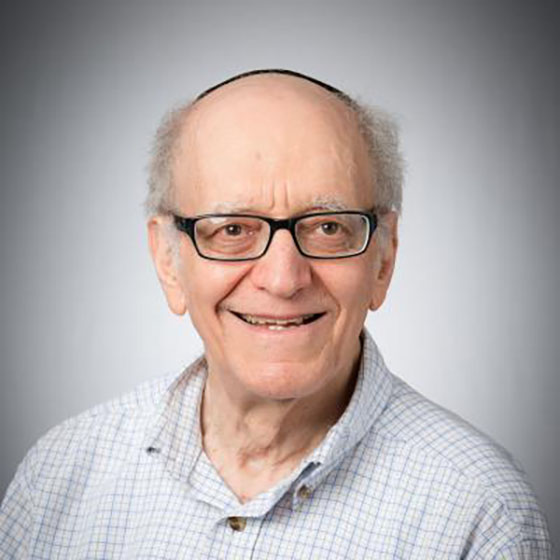
\includegraphics[width=3cm]{Jeff.jpg}
    \end{center}
\end{frame}
\section{Overview}
    \begin{frame}{Overview}
    \begin{itemize}[<+->]
        \item Problem
        \item Key Insights from Original Proof
        \item A Simpler Approach
    \end{itemize}
\end{frame}
\section{Introduction}
    % \input{abstract-vs-concrete}
    \begin{frame}{Computability of Total Functions on $\Reals$}
    \begin{center}
        
\includegraphics[width=.88\linewidth]{total.png}
    \end{center}
\end{frame}
% \begin{frame}{Computability of Partial Functions on $\Reals$}
%     \begin{center}
%         
\includegraphics[width=.88\linewidth]{partial.png}
%     \end{center}
% \end{frame}
\begin{frame}{Computability of Total Functions on $\Reals$}
        \begin{center}
        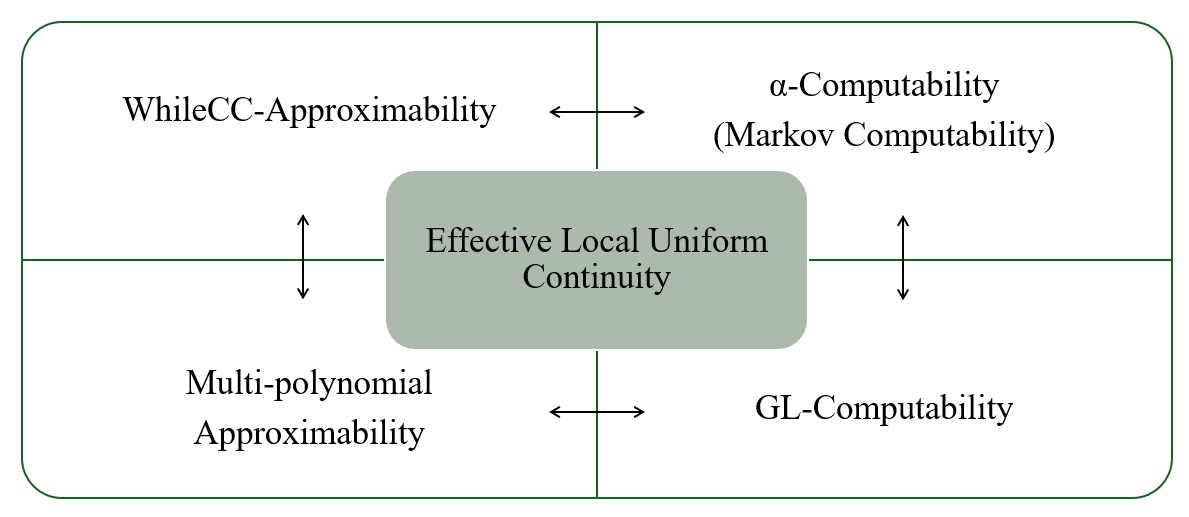
\includegraphics[width=.6\linewidth]{total-zoomed.png}
    \end{center}
\end{frame}

\begin{frame}{Computability of Partial Functions on $\Reals$}
    \textbf{For partial functions on $\Reals$}, \citet{ModelOfCompForPartFunc_MingQuanFuAndJeffZucker} generalize effectively locally uniform continuity to \textbf{\textcolor{violet}{acceptability}} to get an equivalence.\\
    \pause
     \begin{exampleblock}{\textbf{\textcolor{BrickRed}{Problem}}}
        How general is this class of acceptable functions?
     \end{exampleblock}
     \pause
    \begin{center}
        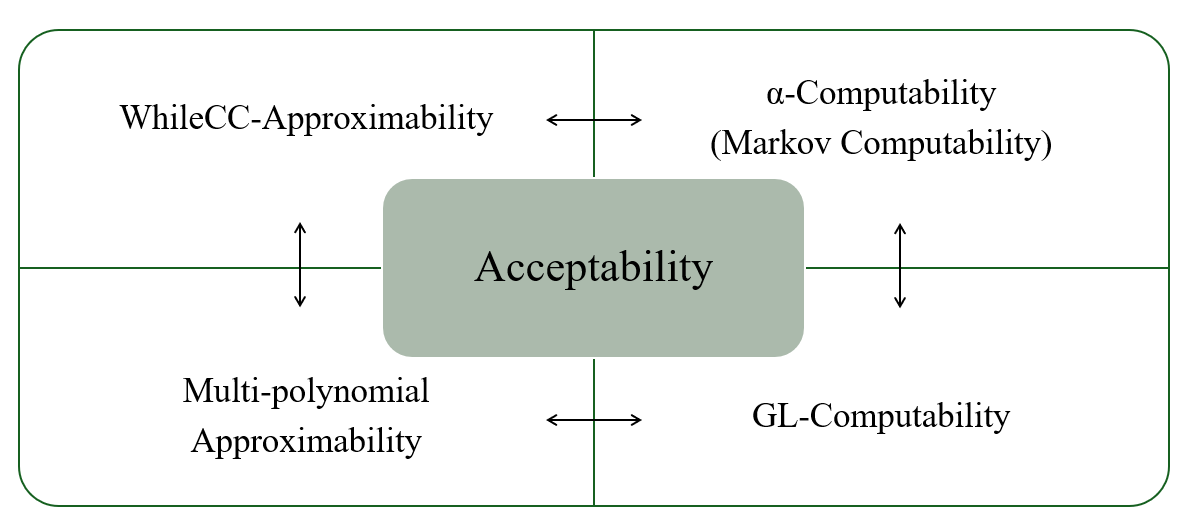
\includegraphics[width=.6\linewidth]{partial-zoomed.png}
    \end{center}
     \begin{exampleblock}{\color{OliveGreen}\textbf{Useful First Step Towards Solution}}
         Show that the elementary functions satisfy the acceptability conditions. 
     \end{exampleblock}
\end{frame}


 
    % \input{problem}
\section{Background}
    % \input{whilecc}
    
\begin{frame}{Background -- Acceptability}
    \begin{definition}[\textbf{\textcolor{violet}{Acceptability}}]
        A function $f:\Reals\to\Reals$ is \textbf{\textcolor{violet}{acceptable}} if there exists a sequence $X$ where:
        \begin{enumerate}
            \pause\item $X$ is an  \textbf{\textcolor{olive}{effective open exhaustion}} for $\dom(f)$, and
            \pause\item $f$ is  \textbf{\textcolor{brown}{effectively locally uniformly continuous w.r.t.\null{} $X$}}.
        \end{enumerate}
    \end{definition}
\end{frame}
\begin{frame}{Background -- Effective Open Exhaustions}
\vspace{-1em}
\pause
\begin{definition}[\citep{ModelOfCompForPartFunc_MingQuanFuAndJeffZucker}]
        \pause A sequence $(U_1, U_2, \ldots)$ of open sets is called an \textbf{\textcolor{olive}{effective open exhaustion}} for an open $U\subseteq \Reals$ if 
        \pause \begin{enumerate}
                \item $ U = \bigcup_{l=0}^\infty U_l$, and
                \pause\item for each $l \in \Nats$,
                  $U_l$ \pause is a finite union of non-empty open finite intervals $I_1^l, I_2^l,...,I_{k_l}^l $ whose closures are pairwise disjoint, and
                \pause\item for each $l \in \Nats$,
                   $\overline{U_l} = \bigcup_{i=1}^{k_l} \overline{I_i^l} \subseteq U_{l+1}$.
                \pause\item 
                for all $l$, the components $I_i^l$ that are intervals building up the stage $U_l$, are \textit{rational} \pause and \textit{ordered} i.e., $I_i^l = (a_i^l, b_i^l)$ for some $a_i^l, b_i^l \in \Rationals$ where $b_i^l < a_{i+1}^l$ for $i=1,...,k_l-1$, and
                \pause\item the map
                $l\mapsto ( a_1^l , b_1^l, ...,
                 a_{k_l}^l, b_{k_l}^l)$
                which delivers the sequence of stages $U_l = I_1^l\cup ...\cup I_{k_l}^l$ is recursive.
        \end{enumerate}
    \end{definition}
    \pause
    \begin{itemize}
        \item 
        The sequence of open sets $(-1, 1), (-2, 2), \ldots, (-k, k), \ldots$
        is the standard effective open exhaustion for $\Reals$.
        \pause\item 
        The notion of effective open exhaustions is equivalent to the notion of \textbf{\textcolor{Sepia}{recursively enumerable (r.e./c.e) open sets \citep{Weihrauch2000}}}.
    \end{itemize}
   
\end{frame}
\begin{frame}{Background -- Effective Local Uniform Continuity}
    \pause
    \begin{definition}[\citep{ModelOfCompForPartFunc_MingQuanFuAndJeffZucker}]
        A function $f$ on $U$ is \textbf{ effectively locally uniformly continuous \textbf{\textcolor{BrickRed}{w.r.t.\null{} an effective open exhaustion}}} $(U_n)_{n \in \Nats}$ of $U$, \pause if there is a recursive function $M:\Nats^2\totalTo \Nats$ such that for all $k,l \in \Nats$ and all $x,y \in U_l$:
        \[
        \abs{x-y}<2^{-M(k,l)} \then \abs{f(x)-f(y)}<2^{-k}
        \]    
    \end{definition}
\end{frame}
\section{Problem}
    \begin{frame}{Background -- Elementary Functions}
    \pause \vspace{-2em}
    \begin{minipage}[t]{0.48\linewidth}
        \begin{definition}[%Elementary functions,
                           \citep{OrdinaryDifferentialEquations_Morris_Tenenbaum_1985}]
            The \textbf{elementary functions} on $\Reals$  are partial functions defined by expressions built up from 
            \pause

            \kern-1ex
            \begin{itemize}
                \setlength\itemsep{-1pt}
                \item computable reals, and
                \item the variable $x$,
            \end{itemize}
            \kern-1ex
            \pause by applying (repeatedly) the basic operations below on elementary functions $f,g$:
            \pause
            \begin{itemize}
                \setlength\itemsep{-1pt}
                \item $(f+g)(x) = f(x) + g(x)$ 
                \item $(f\cdot g)(x) = f(x)g(x)$
                \item $\mathrm{inv}_f(x) = \frac{1}{f(x)}$ \kern5em where $\frac{1}{0} =\ \uparrow$
                \item $\mathrm{root}_{n,f}(x) = \sqrt[n]{f(x)}$ \hfill where $0< n \in \Nats$
                \item $\ln_f(x) = \ln(f(x))$
                \item $\exp_f(x) = e^{f(x)}$
                \item $\sin_f(x) = \sin(f(x))$
                \item $\arcsin_f(x) = \arcsin(f(x))$
            \end{itemize}
        \end{definition}
    \end{minipage}
    \hfill
    \pause \begin{minipage}[t]{0.45\linewidth}
        \begin{exampleblock}{\textbf{\textcolor{BrickRed}{Problem}}}
            The domains of elementary functions are not all open!
        \end{exampleblock}
        \pause
        \begin{exampleblock}{\color{OliveGreen}\textbf{Solution: Modifications}}
            \pause
            \begin{itemize}
                \item We define $\sqrt[n]{x} = 0$ for $x < 0$ when $n$ is even.
                \pause \item We extend the definition of $\arcsin(x)$ to be $\frac{\pi}{2}$ for $x > 1$ and to be $-\frac{\pi}{2}$ for $x<-1$.
            \end{itemize}
        \end{exampleblock}
        \centering
        \visible<7->{
        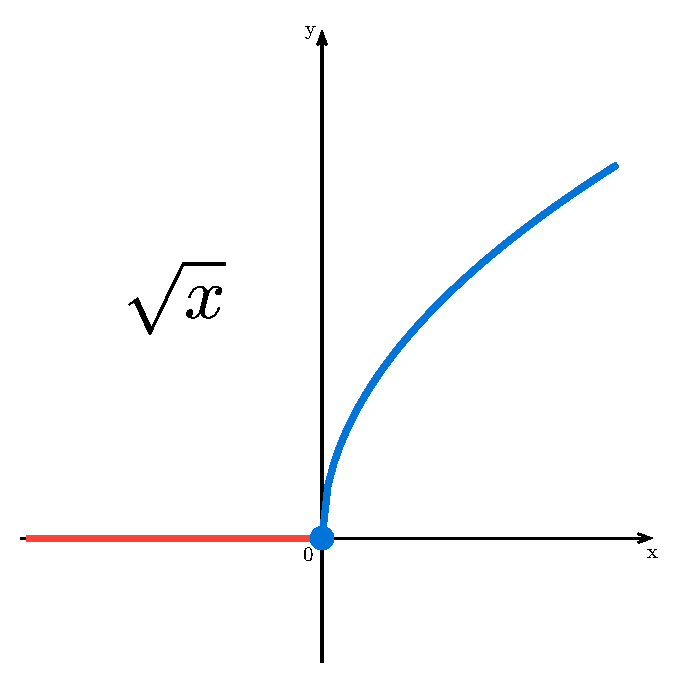
\includegraphics[width=0.35\linewidth]{sqrt.pdf}
        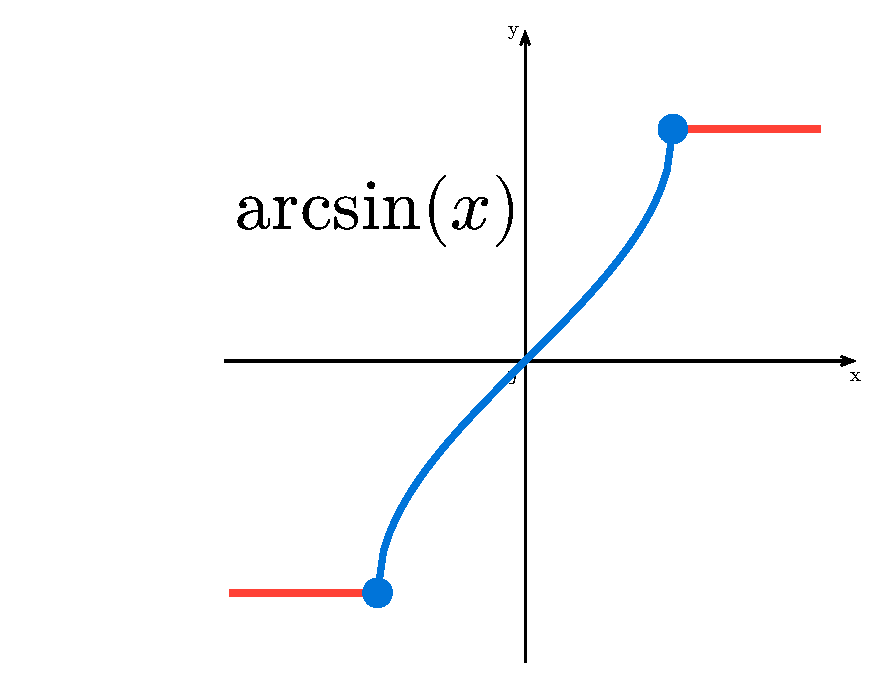
\includegraphics[width=0.35\linewidth]{arcsin.pdf}}
    \end{minipage}\kern-0.2em
\end{frame}
\section{Contributions}
    \begin{frame}{Contributions}
    \vspace{-1em}
    % \begin{exampleblock}
    {\color{gray}
    \textcolor{OliveGreen}{\textbf{Recall: Equivalence Theorem}, \citep{ModelOfCompForPartFunc_MingQuanFuAndJeffZucker}}\\
    For any \textcolor{violet}{acceptable function} $f:\Reals\to\Reals$ and any {effective open exhaustion} $X$ for $\dom(f)$, the following are equivalent:}

    \kern-1ex
        \begin{itemize}
            \setlength\itemsep{-3pt}\color{gray}
            \item $f$ is an $\alpha$-computable function.
            \item $f$ is \textcolor{BrickRed}{\WhileCC-approximable}.
            \item $f$ is GL-computable w.r.t. $X$.
            \item $f$ is effectively locally uniformly multipolynomially approximable w.r.t. $X$.
        \end{itemize}
        
    % \end{exampleblock}
    \pause 
    \begin{ntheorem}[\WhileCC-approximability Theorem](1)
        All elementary functions are \WhileCC-approximable.
    \end{ntheorem}
    \kern1ex
    \pause
    \begin{ntheorem}[Acceptability Theorem](2)
        All elementary functions are acceptable.
    \end{ntheorem}
\end{frame}
\begin{frame}{Contributions}
    \vspace{-1em}
    {\color{gray}
    \textcolor{OliveGreen}{\textbf{Recall: Equivalence Theorem}, \citep{ModelOfCompForPartFunc_MingQuanFuAndJeffZucker}}\\
    For any {acceptable function} $f:\Reals\to\Reals$ and any {effective open exhaustion} $X$ for $\dom(f)$, the following are equivalent:}

    \kern-1ex
        \begin{itemize}
            \setlength\itemsep{-3pt}\color{gray}
            \item $f$ is an $\alpha$-computable function.
            \item $f$ is \WhileCC-approximable.
            \item $f$ is GL-computable w.r.t. $X$.
            \item $f$ is effectively locally uniformly multipolynomially approximable w.r.t. $X$.
        \end{itemize}

    \kern1ex
    \begin{ntheorem}[\WhileCC-approximability Theorem](1)
        All elementary functions are \WhileCC-approximable.
    \end{ntheorem}

    \kern0.5ex
    \begin{ntheorem}[Acceptability Theorem: Part 1](2.1)
        The domain of any elementary function has an effective open exhaustion.
    \end{ntheorem}
    
    \kern0.1ex
    \begin{ntheorem}[Acceptability Theorem: Part 2](2.2)
        Any elementary function is {effectively locally uniformly continuous} w.r.t.\null{} an effective open exhaustion for its domain.
    \end{ntheorem}
\end{frame}

    \begin{frame}{Result 1}
    \pause
    \begin{ntheorem}[\WhileCC-approximability Theorem](1)
        All elementary functions are \WhileCC-approximable.
    \end{ntheorem}
\end{frame}
    \input{Contribution1-wcc-appx}
\section{Challenges}
    % \input{challenges1}
    % \input{challenges1-part1}
    \begin{frame}{Result 2}
    \pause
    \vspace{-1.5em}
    \begin{ntheorem}[Acceptability Theorem: Part 2](2.2)
        Any elementary function is effectively locally uniformly continuous \textbf{\textcolor{BrickRed}{w.r.t.\null{} an effective open exhaustion}} for its domain.
    \end{ntheorem}
    \pause
    \vspace{-0.5em}
    \begin{exampleblock}{\color{OliveGreen}\textbf{(We prove that this is) equivalent to proving:}}
        Any elementary function has a local modulus of continuity.
    \end{exampleblock}
    \pause
    \vspace{-0.5em}
    \begin{definition}[Local modulus of continuity]
        Let $f:\Reals\to\Reals$. A recursive function $N:\Rationals\times\Rationals\times\Nats\to\Nats$ is called a \textbf{local modulus of continuity} for $f$\index{local modulus of continuity} iff for any $a,b\in\Rationals$ with $[a,b]\subseteq\dom(f)$ and $k\in\Nats$, we have
        \[ 
            \forall x,y \in (a,b) \quad \abs{x-y}<2^{-N(a,b,k)} \then \abs{f(x)-f(y)}<2^{-k}.
        \] 
    \end{definition}
    \pause
        {\textbf{\textcolor{OliveGreen}{The notion of effective local uniform continuity is independent
                of effective open exhaustion.}}}
\end{frame}
\section{Summary and Future Work}
    \begin{frame}{Summary}
    We proved that:
    \pause
    \begin{itemize}
        \item all elementary functions are \WhileCC-approximable.
        \pause \item all elementary functions are acceptable.
    \end{itemize}
     \pause We also 
    \begin{itemize}
         \item  presented an \textbf{alternative characterization} of acceptable functions \pause using the \textbf{local modulus of continuity} concept.
    \end{itemize}
\end{frame}

    \begin{frame}{Alternative Approach}
    \pause
    \begin{theorem}
        The following are true for any function $f$ on the reals:
        \begin{itemize}
            \item 
            {$f$ is GL-computable $\Rightarrow$ $f$ is effectively uniformly continuous w.r.t.\null{} any compact set [Anonymous Reviewer].}
            \pause \item 
            {$f$ is GL-computable + has an r.e. open domain $\Rightarrow$ $f$ is effectively uniformly continuous \citep{pauly2016}.}
        \end{itemize}

    \end{theorem}
    \pause
    \begin{theorem}
            Elementary functions are GL-computable and have open domains.
    \end{theorem}
    \pause
    \begin{proof}
            Straightforward proof by induction.
    \end{proof}
    \pause
    \begin{corollary}
            Elementary functions are acceptable.
    \end{corollary}
\end{frame}
    \begin{frame}{Future Work}

    \pause \textbf{Conjecture:}
    \begin{itemize}
        \item All partial unary \WhileCC-approximable functions are acceptable.
        % \textbf{More Questions:}
        \begin{itemize}
            \pause \item \textbf{If the conjecture holds}, are \emph{non-unary} \WhileCC-approximable functions acceptable?
            \pause \item  \textbf{If not}, what is a model of computation that characterizes exactly the class of acceptable functions?
        \end{itemize}
    \end{itemize}
    \pause
    Also, we would like to know if acceptability is the weakest condition that can be used to prove the equivalence theorem.
    % \pause
    % \textbf{\textcolor{orange}{More Questions Left Unanswered:}}
    % \begin{center}
    %     \vspace{-1em}
    %     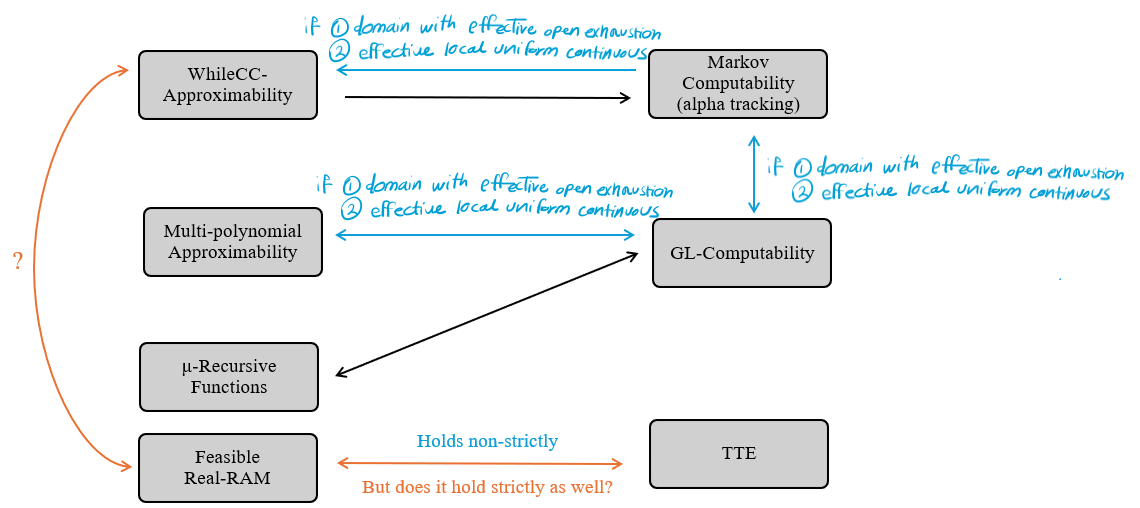
\includegraphics[width=.7\linewidth]{todo.png}
    % \end{center}
\end{frame}
    \input{references}
    \input{thanks}
\end{document}
